\chapter{Bandstructure Modifications}

\section{Bandstructure of Semiconductor Alloys}
One of the simplest and most effective methods to alter the electronic properties of a material or to engineer entirely new properties is through the formation of alloys. Alloying has long been employed across various material classes—not only semiconductors, but also metals and insulators—as a technique to tailor physical and chemical characteristics.

In the context of semiconductors, the motivation to create alloys is typically driven by two primary goals:

\begin{enumerate}
	\item \textit{Tuning the bandgap}: This is particularly important in the design of light-emitting and light-detecting devices, where the bandgap dictates the energy (and thus the wavelength) of the absorbed or emitted photons.
	\item \textit{Lattice constant engineering}: Alloying allows for the synthesis of materials with desired lattice parameters, enabling lattice matching (or deliberate mismatch) with available substrates. For instance, the InGaAs alloy is frequently used because it can be lattice-matched to InP substrates, which are commercially available.
\end{enumerate}
\begin{center}
	\begin{minipage}{0.7\textwidth}
		\centering
		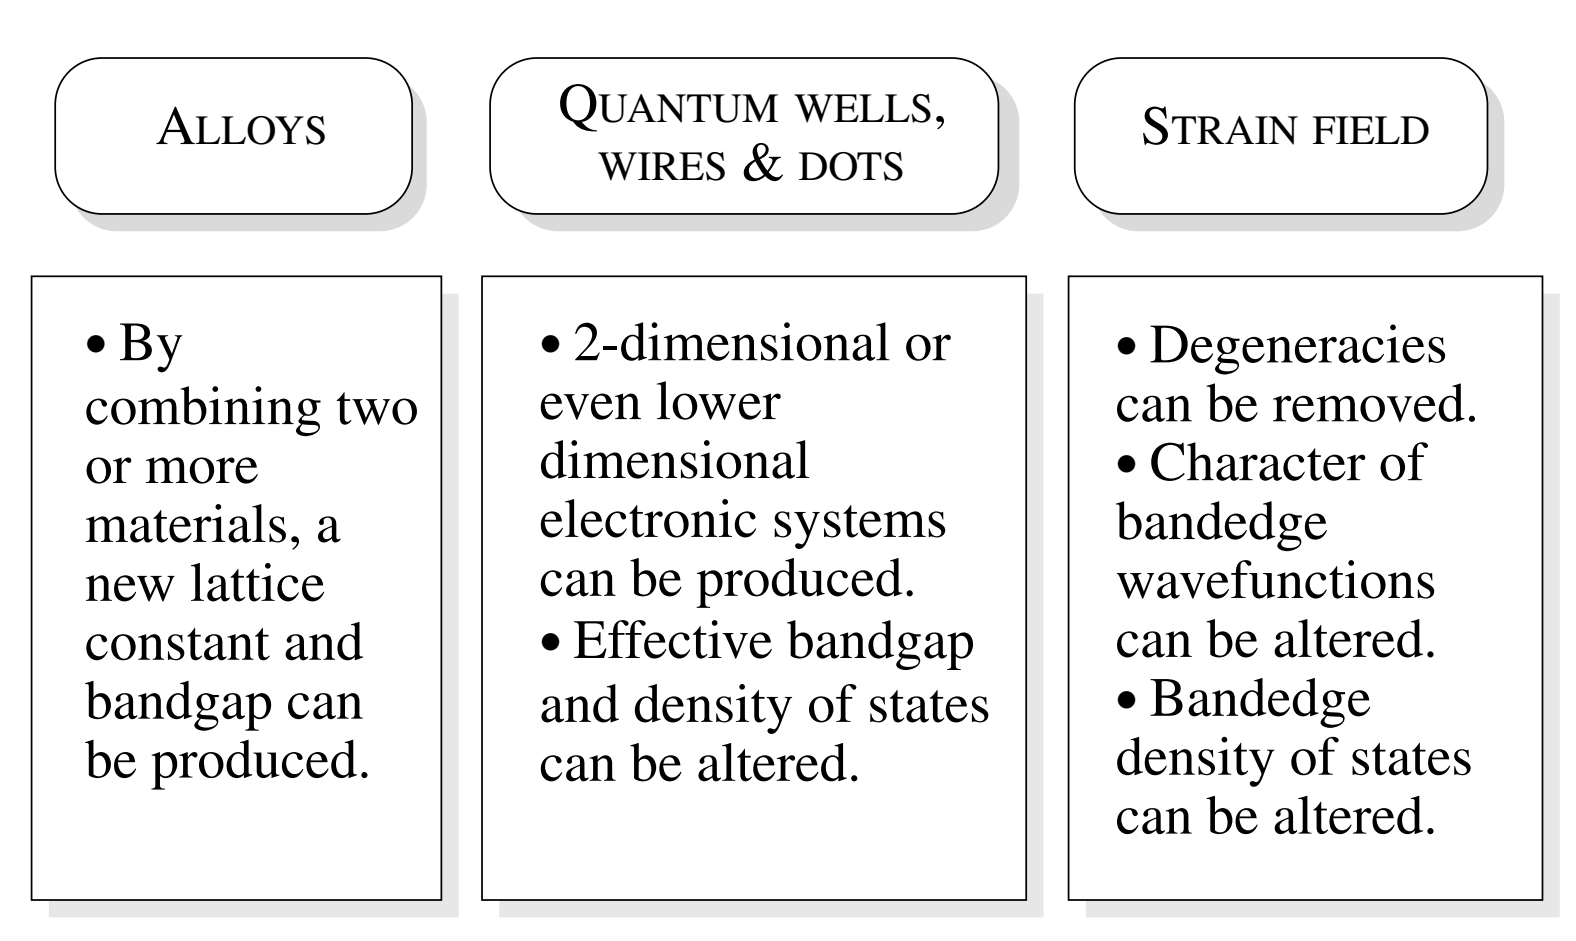
\includegraphics[width=\textwidth]{img/Approaches_BandStructureMod.png}
		\\[0.5em]
		\refstepcounter{figure}
		\textbf{Figure~\thefigure.} Different approaches to modify Bandstructure of semiconductors.
		\label{fig:Approaches_BandStructureMod}
	\end{minipage}
\end{center}
When an alloy of the form \( A_{x}B_{1-x} \) is produced via random mixing of two components \( A \) and \( B \) (a concept that can be generalized to multicomponent systems), the lattice constant of the resulting alloy is often estimated using Vegard's law:
\[
	a_{\text{alloy}} = x a_A + (1 - x) a_B
\]
This empirical relationship assumes a linear interpolation between the lattice constants \( a_A \) and \( a_B \) of the pure materials and is valid for random alloys where no phase separation occurs and both components share the same crystal structure.
The term "random" in this context refers to the statistical distribution of atoms within the alloy. Specifically, in a random alloy, the probability that a given atomic site is occupied by atom \( A \) is \( x \), while the probability that it is occupied by atom \( B \) is \( 1 - x \). However, several distinct atomic arrangements are theoretically possible when forming such an alloy:
\begin{enumerate}
	\item \textit{Phase separation}: Atoms of type \( A \) cluster together in one region, while atoms of type \( B \) cluster in another, forming distinct domains of the pure components.
	\item \textit{Random distribution}: Each atomic site is occupied according to the probability \( x \) for \( A \) and \( 1 - x \) for \( B \), independent of neighboring sites.
	\item \textit{Ordered structure}: Atoms \( A \) and \( B \) arrange themselves in a well-defined periodic pattern, forming a superlattice.
\end{enumerate}
\begin{center}
	\begin{minipage}{0.4\textwidth}
		\centering
		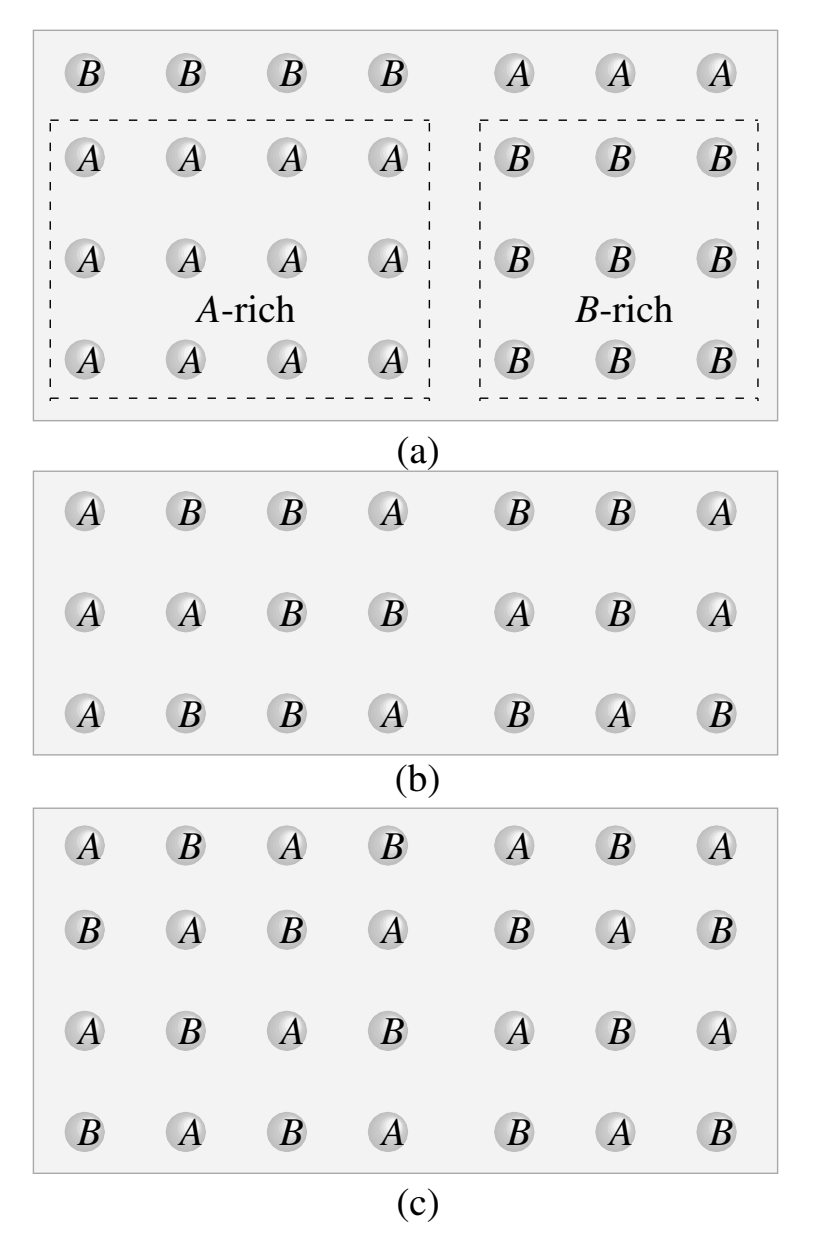
\includegraphics[width=\textwidth]{img/clustered-ordered-ordered.png}
		\\[0.5em]
		\refstepcounter{figure}
		\textbf{Figure~\thefigure.} A schematic example of (a) a clustered, (b) a random, and (c) an ordered alloy structure.
		\label{fig:clustered-ordered-ordered}
	\end{minipage}
\end{center}

In practice, most semiconductor alloys used in modern electronic and optoelectronic applications are synthesized with the goal of producing statistically random distributions of constituent atoms. Such random alloys provide the desired combination of bandgap tunability and structural compatibility with various substrates.\\
Alloys typically retain a well-defined crystal structure; however, the random occupation of lattice sites by different atomic species eliminates the strict periodicity of the background potential—except in the case of ordered alloys or superlattices. As a result, Bloch’s theorem no longer applies, and the electronic wavefunctions can no longer be represented as simple traveling waves. Instead, they become more complex, exhibiting spatially varying probability distributions.
To make progress in understanding the bandstructure of such disordered systems, a commonly employed approximation is the \textit{virtual crystal approximation} (VCA). This approach replaces the spatially random potential experienced by the electrons with an averaged periodic potential:
\begin{equation}
	U_{\text{av}}(\mathbf{r}) = x U_A(\mathbf{r}) + (1 - x) U_B(\mathbf{r})
\end{equation}
Here, \( U_A \) and \( U_B \) are the atomic potentials of the two constituent species, and \( x \) represents the concentration of species \( B \). The VCA allows one to treat the alloy as if it were a periodic crystal with an effective potential.
In practical implementations—such as within the tight-binding method—this corresponds to averaging the matrix elements of the Hamiltonian. For direct bandgap semiconductors, where the conduction and valence band edges occur at the \(\Gamma\)-point (i.e., \( \mathbf{k} = 0 \)), the bandgap is also approximated by a linear interpolation:
\begin{equation}
	E_g^{\text{alloy}} = x E_g^A + (1 - x) E_g^B
\end{equation}
However, in many real materials, this linear relationship is not sufficient due to a phenomenon known as \textit{bandgap bowing}. This deviation arises from the increasing disorder and complex interactions introduced by alloying. A more accurate empirical expression for the bandgap is:
\begin{equation}
	E_g^{\text{alloy}} = a + bx + c x^2
\end{equation}
where \( a \), \( b \), and \( c \) are material-specific constants, and \( c \) is known as the bowing parameter.
In addition to bandgap behavior, the effective masses at the band edges also vary with composition. Within the VCA, the effective mass of the alloy can be approximated by:
\begin{equation}
	\frac{1}{m^*_{\text{alloy}}} = \frac{x}{m^*_A} + \frac{1 - x}{m^*_B}
\end{equation}
This follows from the expression for the energy dispersion near the band edge, assuming parabolic bands:
\begin{equation}
	E_{\text{alloy}}(k) = x \frac{\hbar^2 k^2}{2 m^*_A} + (1 - x) \frac{\hbar^2 k^2}{2 m^*_B}
\end{equation}
Several important alloy systems have played critical roles in advancing semiconductor electronics and optoelectronics. These will be briefly discussed in the following sections.
\begin{center}
	\begin{minipage}{0.9\textwidth}
		\centering
		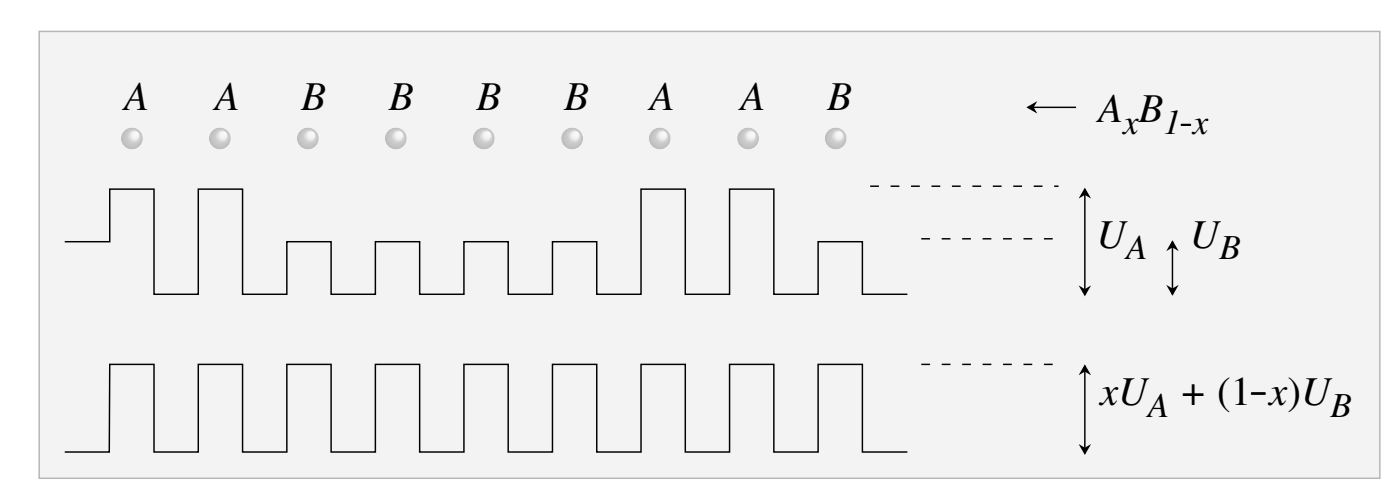
\includegraphics[width=\textwidth]{img/VCA.png}
		\\[0.5em]
		\refstepcounter{figure}
		\textbf{Figure~\thefigure.} Motivation for the virtual crystal approximation (VCA). The top part illustrates a lattice with A- and B-type atoms, each associated with localized potentials $U_A$ and $U_B$. In the VCA, extended states experience an effective periodic potential given by the weighted average $xU_A + (1 - x)U_B$.
		\label{fig:VCA}
	\end{minipage}
\end{center}

\subsection{GaAs/AlAs Alloy}
The AlGaAs system is among the most important and widely studied semiconductor alloy systems. A key advantage of this system is that AlAs and GaAs are nearly lattice matched, allowing the alloy \( \text{Al}_x\text{Ga}_{1-x}\text{As} \) to be epitaxially grown on GaAs substrates without the buildup of significant strain energy. This lattice compatibility makes AlGaAs highly suitable for the fabrication of high-speed electronic and optoelectronic devices.\\
In electronic applications, AlGaAs plays a central role in the development of modulation-doped field-effect transistors (MODFETs), while in optoelectronics it is used in a variety of devices such as modulators, photodetectors, and laser diodes.\\
One particularly noteworthy property of the AlGaAs alloy system is the compositional dependence of its electronic band structure, specifically the nature of its bandgap. As the aluminum content increases, the conduction band minimum transitions from the \(\Gamma\)-valley to the \(X\)-valley, resulting in a switch from a direct to an indirect bandgap.\\
This transition typically occurs when the aluminum mole fraction exceeds approximately 35\%. Consequently, for most optoelectronic device applications that require efficient radiative recombination (i.e., direct bandgap), the aluminum composition is chosen to be below this threshold.\\
This compositional dependence of the conduction band valleys is critical in determining the optical and electronic properties of AlGaAs-based devices and must be carefully accounted for in device design and material synthesis.
\begin{center}
	\begin{minipage}{0.7\textwidth}
		\centering
		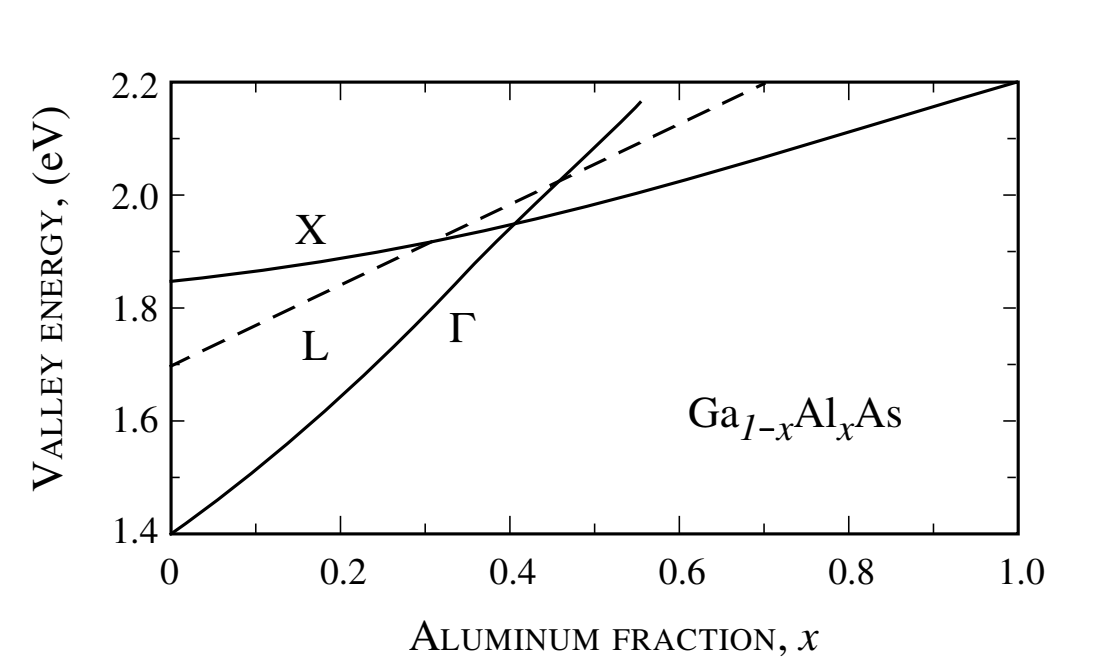
\includegraphics[width=\textwidth]{img/AlGaAs.png}
		\\[0.5em]
		\refstepcounter{figure}
		\textbf{Figure~\thefigure.} The variation of conduction band valleys in AlGaAs as a function of composition at 300 K.
		\label{fig:AlGaAs}
	\end{minipage}
\end{center}

\section{Bandstructure Modifications by Heterostructures}
It is possible to vary the chemical composition of a semiconductor structure along the growth direction using advanced epitaxial techniques such as molecular beam epitaxy (MBE) or metal-organic chemical vapor deposition (MOCVD). By introducing compositionally distinct layers, one can fabricate heterostructures capable of confining electronic states, thereby creating lower-dimensional systems. These systems are now widely utilized in high-performance optoelectronic and electronic devices.\\
Considerable effort has been devoted to extending confinement from one dimension (quantum wells) to two-dimensional (quantum wires) and three-dimensional (quantum dots) systems. While confinement in one dimension is conceptually straightforward and technologically mature, achieving confinement in additional directions often requires complex and challenging epitaxial or post-growth processing techniques.\\
As previously discussed, strained epitaxy can lead to the formation of self-assembled quantum dots, which serve as quasi-zero-dimensional (0D) systems. These have enabled the development of novel device architectures. Although our focus will remain primarily on quantum wells, we will also highlight key considerations related to quantum dots.\\
When two semiconductors are joined to form a heterostructure, one of the most critical questions is how the band edges of the two materials align at the interface. Suppose material \( A \) has a bandgap \( E_g^A \), conduction band edge \( E_c^A \), and valence band edge \( E_v^A \), and material \( B \) has a bandgap \( E_g^B \), with corresponding band edges \( E_c^B \) and \( E_v^B \). Several distinct band alignments may arise depending on the specific materials used.\\
In semiconductor physics, it is common to use electron affinity (or work function) to estimate how the conduction or valence bands align. However, this approach often fails for real heterojunctions due to complex interfacial effects such as charge transfer and atomic bonding. As a result, accurate determination of band lineups usually relies on experimental measurements, though theoretical predictions can often capture general trends.
Three main types of band alignments are typically observed:
\begin{itemize}
	\item \textbf{Type I (Straddling gap):} Both the conduction band minimum and valence band maximum of the narrower-gap material lie within the bandgap of the wider-gap material. This allows both electrons and holes to be confined in the same region. Common examples include GaAs/AlGaAs, InGaAs/InP, and GaN/AlGaN systems.
	\item \textbf{Type II (Staggered gap):} The conduction band minimum lies in one material while the valence band maximum lies in the other. Although this configuration may lead to a small effective bandgap, the spatial separation of carriers weakens optical transitions. Antimonide-based systems such as InSb and GaSb often exhibit type II alignment. The InAs/GaSb system is a well-known example.
	\item \textbf{Broken gap:} In some cases, the conduction band of one material lies below the valence band of the other. These are sometimes referred to as broken gap type II heterostructures.
\end{itemize}
\begin{center}
	\begin{minipage}{0.8\textwidth}
		\centering
		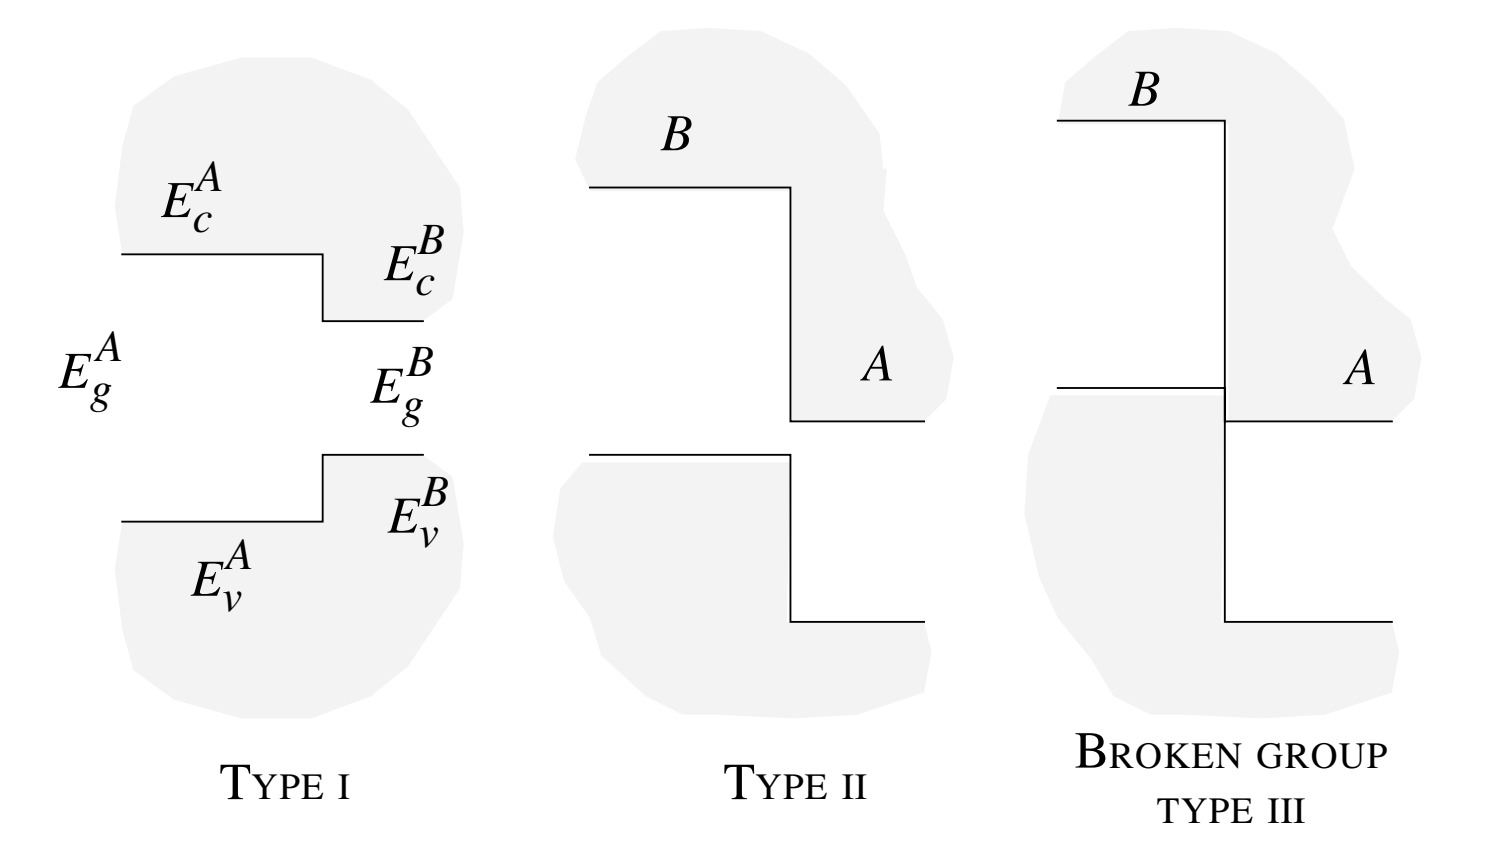
\includegraphics[width=\textwidth]{img/Bandledge_heterostructure.png}
		\\[0.5em]
		\refstepcounter{figure}
		\textbf{Figure~\thefigure.} Various possible bandedge lineups in heterostructure.
		\label{fig:Bandledge_heterostructure}
	\end{minipage}
\end{center}
Once the band alignment is determined, the next step is to describe the electronic states in the heterostructure. A widely used method for this purpose is the \textit{k·p} approach. In its simplest form, the Schrödinger equation for a carrier in a heterostructure can be approximated as:
\begin{equation}
	\left[ -\frac{\hbar^2}{2 m_0} \nabla^2 + V(\mathbf{r}) \right] \psi(\mathbf{r}) = E \psi(\mathbf{r})
	\quad \Rightarrow \quad
	\left[ -\frac{\hbar^2}{2 m^*} \nabla^2 + E_{\text{edge}} \right] \phi = E \phi
\end{equation}
Here, the atomistic potential \( V(\mathbf{r}) \) is replaced by the band-edge energy \( E_{\text{edge}} \), and the complex effect of the crystal environment is incorporated into the effective mass \( m^* \). This simplification forms the basis for the envelope function approximation commonly used in modeling quantum wells and other heterostructures.


\subsection{Bandstructure in Quantum Wells}
To calculate the bandstructure in quantum wells, it is essential to understand the nature of the energy levels and wavefunctions near the edges of the bandgap, as these determine the electronic states in the quantum well. We consider the case where the well region is composed of a direct bandgap semiconductor. In such systems, the conduction band states are primarily of $s$-type character, while the valence band states are $p$-type. Although the formalism can be extended to other material systems, we focus here on a basic quantum well structure.\\
The Schrödinger equation describing the electron states in the quantum well, within the effective mass approximation, is given by:
\begin{equation}
	\left[-\frac{\hbar^2}{2 m^*} \nabla^2 + V(z) \right] \Psi = E \Psi
\end{equation}
Here, \( m^* \) is the effective mass of the electron, and \( V(z) \) is the quantum well potential, which depends only on the growth direction \( z \). The total wavefunction can be separated into its in-plane and out-of-plane components:
\begin{equation}
	\Psi(x, y, z) = e^{i(k_x \cdot x + k_y \cdot y)} f(z)
\end{equation}
\begin{center}
	\begin{minipage}{0.6\textwidth}
		\centering
		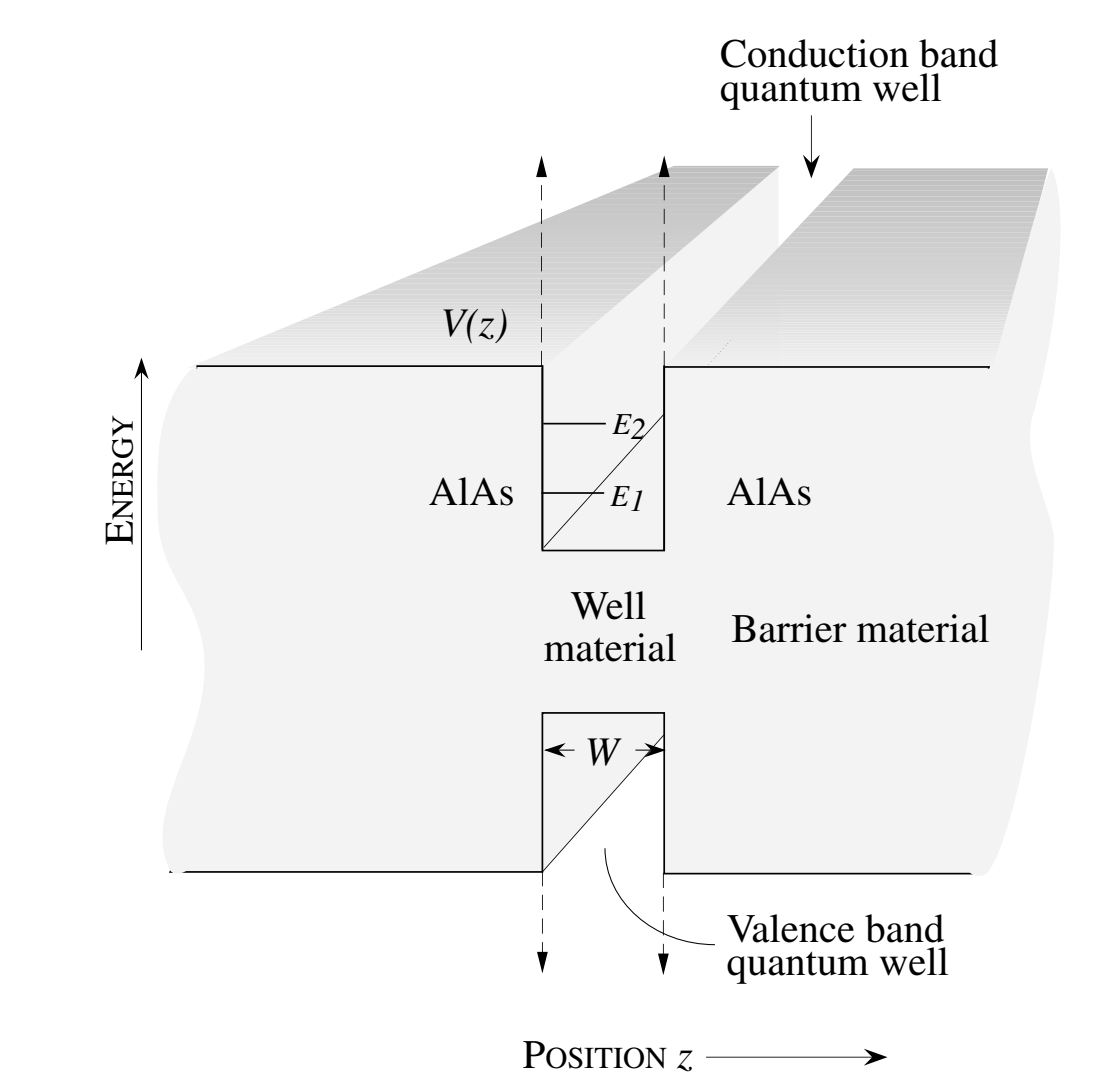
\includegraphics[width=\textwidth]{img/quantum_well_heterostructure.png}
		\\[0.5em]
		\refstepcounter{figure}
		\textbf{Figure~\thefigure.} A quantum well formed for the electron and holes in a heterostructure.
		\label{fig:quantum_well_heterostructure}
	\end{minipage}
\end{center}
Substituting this into the Schrödinger equation yields a one-dimensional equation for \( f(z) \):
\begin{equation}
	\left[-\frac{\hbar^2}{2 m^*} \frac{\partial^2}{\partial z^2} + V(z) \right] f(z) = E_n f(z)
\end{equation}
This one-dimensional quantum well problem is standard and can be found in many undergraduate quantum mechanics texts. Assuming infinite potential barriers, the wavefunctions are:
\[
	f_n(z) =
	\begin{cases}
		\cos\left( \frac{n \pi z}{W} \right), & \text{if } n \text{ is even} \\
		\sin\left( \frac{n \pi z}{W} \right), & \text{if } n \text{ is odd}
	\end{cases}
\]
where \( W \) is the well width. The corresponding quantized energy levels are:
\begin{equation}
	E_n = \frac{\pi^2 \hbar^2 n^2}{2 m^* W^2}
\end{equation}
Including the in-plane kinetic energy contribution, the total energy of the electron becomes:
\begin{equation}
	E(k) = E_n + \frac{\hbar^2 k_\parallel^2}{2 m^*}
\end{equation}
This results in subbands within the conduction and valence bands. If the potential barrier \( V \) is finite, the wavefunction decays exponentially into the barrier region. The solution inside the well remains sinusoidal, but matching boundary conditions leads to the transcendental equations:
\begin{equation}
	\alpha \tan\left( \frac{\alpha W}{2} \right) = \beta \quad \text{or} \quad \alpha \cot\left( \frac{\alpha W}{2} \right) = -\beta
\end{equation}
where
\begin{equation}
	\alpha = \sqrt{\frac{2 m^* E}{\hbar^2}}, \quad \beta = \sqrt{\frac{2 m^* (V_c - E)}{\hbar^2}}
\end{equation}
These equations can be solved numerically to obtain the quantized energy levels \( E_1, E_2, E_3, \dots \), each corresponding to a subband in the quantum well.\\
In the valence band, both heavy hole and light hole subbands exist, and their detailed dispersion relations are affected by strain and confinement. The resulting subband structure plays a significant role in determining the optical and transport behavior of heterostructures.\\
An important consequence of the subband formation is its impact on the density of states (DOS), which influences both optical absorption and carrier dynamics.

For a quantum well, the DOS in the conduction band is:
\begin{equation}
	N(E) = \sum_i \frac{m_i^*}{\pi \hbar^2} \, \sigma(E - E_i)
\end{equation}
where \( \sigma \) is the Heaviside step function and \( E_i \) are the subband energies.

For the valence band, including both heavy and light hole contributions, the DOS becomes:
\begin{equation}
    N(E) = \sum_i \sum_{j=1}^{2} \frac{m_j^*}{\pi \hbar^2} \, \sigma(E_{ij} - E)
\end{equation}
Here, \( j = 1 \) denotes heavy holes and \( j = 2 \) denotes light holes, and \( m_{ij}^* \) are the respective effective masses.\\
In the simplified model described here, the conduction band state is assumed to be purely $s$-type, and a basic effective mass approximation is used. More sophisticated calculations can incorporate full-band models, such as eight-band \textit{k·p} theory, which captures coupling between conduction and valence bands. For unstrained structures, such enhancements do not significantly alter the conduction subband energies. However, for strained heterostructures, a more complete bandstructure model becomes necessary.

\begin{center}
	\begin{minipage}{0.8\textwidth}
		\centering
		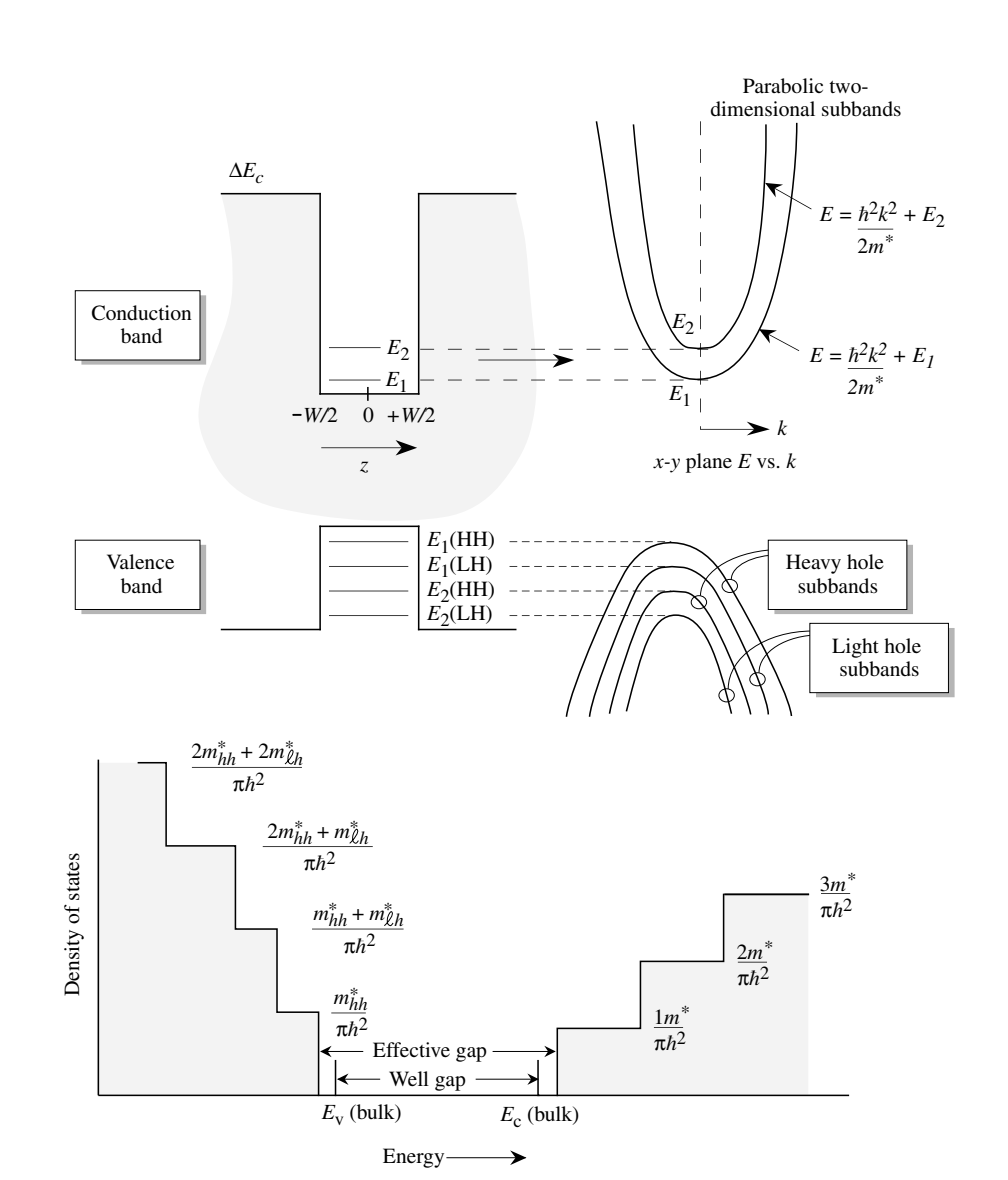
\includegraphics[width=\textwidth]{img/DensityOfState.png}
		\\[0.5em]
		\refstepcounter{figure}
		\textbf{Figure~\thefigure.} Density of states in a 3-, 2-, and 1-dimensional system with a parabolic energy momentum relations.
		\label{fig:DensityOfState}
	\end{minipage}
\end{center}

\subsection{Valence Bandstructure in Quantum Wells}
The description of quantum well bandstructure and density of states outlined earlier is quite accurate for electron states. This is because, in direct bandgap semiconductors, the conduction band is derived predominantly from an $s$-type orbital, and can therefore be treated as a single non-degenerate band. \\
However, the valence band states arise from $p$-type orbitals, leading to the formation of heavy-hole (HH) and light-hole (LH) bands. While the HH states (with total angular momentum $j = 3/2$, $m_j = \pm 3/2$) and LH states ($j = 3/2$, $m_j = \pm 1/2$) are pure and uncoupled at $k = 0$, they exhibit strong mixing as one moves away from the Brillouin zone center.\\
For the purpose of determining subband energy levels, the starting energies can still be calculated separately for HH and LH bands, similarly to the electron case. However, the in-plane ($k_x$–$k_y$) dispersion of hole states is only approximately given by a simple parabolic relation:
\begin{equation}
	E(\mathbf{k}) = E_{n,i} + \frac{\hbar^2 k^2}{2 m_i^*}
\end{equation}
where $i$ denotes either the HH or LH band. A more accurate description of the valence band structure is obtained by solving the Kohn–Luttinger form of the Schrödinger equation:
\begin{equation}
	[H + V_p(z)] \Psi = E \Psi
\end{equation}
Here, $H_p$ is the Kohn–Luttinger Hamiltonian, which in the case of HH and LH coupling becomes a $4 \times 4$ matrix differential operator. Treating the out-of-plane momentum as an operator ($k_z = -i \partial / \partial z$), we obtain the following forms for the Hamiltonian matrix elements:
\begin{equation}
	H_{\text{hh}} = -\frac{\hbar^2}{2m_0} \left[ (\gamma_1 + \gamma_2)(k_x^2 + k_y^2) - (\gamma_1 - 2\gamma_2) \frac{\partial^2}{\partial z^2} \right] + V_p(z)
\end{equation}
\begin{equation}
	H_{\text{lh}} = -\frac{\hbar^2}{2m_0} \left[ (\gamma_1 - \gamma_2)(k_x^2 + k_y^2) - (\gamma_1 + 2\gamma_2) \frac{\partial^2}{\partial z^2} \right] + V_p(z)
\end{equation}
\begin{equation}
	c = \sqrt{3} \frac{\hbar^2}{2 m_0} \left[\gamma_2(k_x^2 - k_y^2)- 2 i \gamma_3 k_x k_y\right]
\end{equation}
\begin{equation}
	b = -i \sqrt{3} \frac{\hbar^2}{m_0} \gamma_3 (- k_y - i k_x) \frac{\partial}{\partial z}
\end{equation}
In these expressions, $V(z)$ represents the quantum well confinement potential, and $\gamma_1$, $\gamma_2$, and $\gamma_3$ are the Luttinger parameters describing the anisotropic hole mass.\\
When biaxial strain is present, additional terms must be included in the Hamiltonian to account for strain-induced modifications in the band structure. These will be introduced in later sections.
The general form of the hole wavefunction can be written as:
\begin{equation}
	\Psi^m_{h}(\mathbf{k}_\parallel,z) = \sum_v g^m_v(z) \, U^v(\mathbf{r}) \, e^{i \mathbf{k}_\parallel \cdot \boldsymbol{\rho}}
\end{equation}
Here, $g^m_v(z)$ are envelope functions that depend on the confinement potential along the growth direction, $U^v(\mathbf{r})$ are the bulk valence band Bloch functions, $m$ is the subband index, and $v$ labels the spinor components associated with the total angular momentum $j = 3/2$ states.\\
This formalism provides a more complete and accurate picture of the valence band substructure in quantum wells, particularly when dealing with hole transport, optical transitions, and strain-induced effects.


\section{Strain and Deformation Potential Theory}
The influence of strain on the electronic and optical properties of semiconductors has been studied extensively over several decades. These investigations have been critical for developing a deeper theoretical understanding of semiconductor bandstructure, particularly by identifying the symmetry properties of energy states involved in optically observed transitions.\\
In addition, strain studies have provided valuable insights into the determination of deformation potentials, which play a fundamental role in describing electronic transport under the influence of lattice scattering. Traditionally, strain was introduced into semiconductors through external mechanical means, often employing sophisticated tools such as diamond anvil cells. These experiments were primarily focused on elucidating the fundamental physics of semiconductors.\\
With the development of strained heteroepitaxy, it has become possible to incorporate strain directly during the epitaxial growth process. Remarkably, built-in strains of a few percent can now be achieved simply by depositing a film onto a substrate with a mismatched lattice constant, as discussed in prior sections.\\
Once the strain tensor is known, the deformation potential theory can be employed to compute the effect of strain on the electronic states throughout the Brillouin zone. The perturbation Hamiltonian due to strain is introduced and analyzed within the framework of first-order perturbation theory. It is generally expressed as:
\begin{equation}
	H_{ij} = \sum_{\alpha\beta} D_{ij}^{\alpha\beta} \, \varepsilon_{\alpha\beta}
\end{equation}
Here, \( D_{ij}^{\alpha\beta} \) are the matrix elements of the deformation potential tensor \( D_{ij} \), and \( \varepsilon_{\alpha\beta} \) are the components of the strain tensor. The deformation potential operator \( D_{ij} \) transforms as a second-rank tensor under the crystal’s symmetry operations.\\
This formalism provides a powerful and practical framework for quantifying the influence of strain on semiconductor electronic structure, and is widely used in the analysis
\begin{center}
	\begin{minipage}{0.7\textwidth}
		\centering
		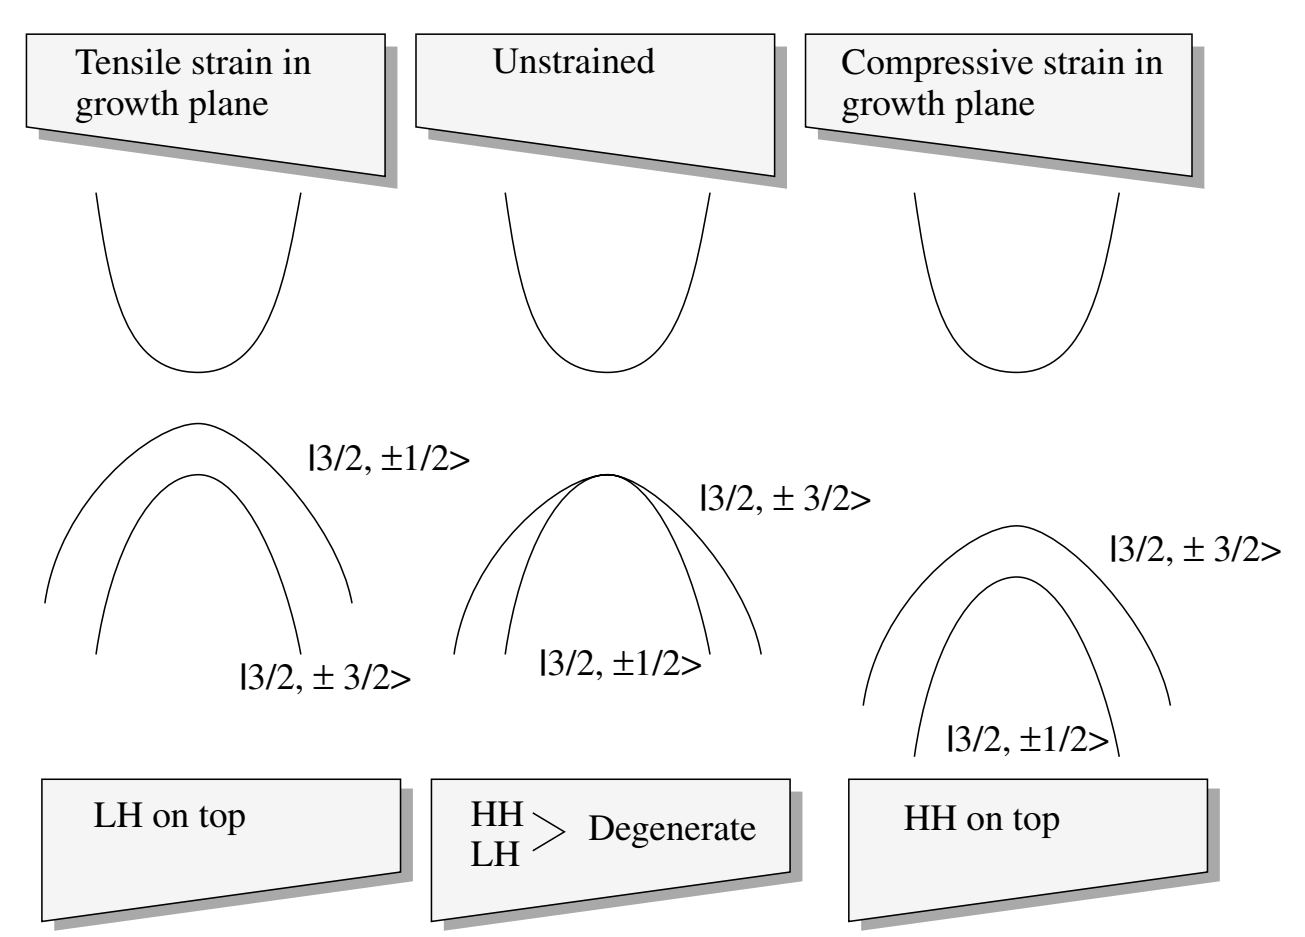
\includegraphics[width=\textwidth]{img/strain_effect.png}
		\\[0.5em]
		\refstepcounter{figure}
		\textbf{Figure~\thefigure.} The effect of strain on the bandstructure of a semiconductor. The conduction band minimum (CBM) and valence band maximum (VBM) shift in response to applied strain. \\
		\label{fig:strain_effect}
	\end{minipage}
\end{center}

Strain introduced in a semiconductor layer grown along the (001) crystallographic direction can significantly modify the band structure, particularly near the band edges. In the case of a direct bandgap semiconductor, the conduction band edge shifts upward or downward relative to its unstrained position, depending on the nature of the strain. However, since the conduction band minimum is typically a non-degenerate state, no splitting occurs under strain.\\
In contrast, the valence band edge is degenerate in the unstrained bulk system. Even in unstrained quantum wells, quantum confinement alone can lift this degeneracy between heavy-hole (HH) and light-hole (LH) states. However, the resulting energy splitting is usually modest, typically on the order of 10–15~meV.\\
When biaxial strain is applied, the impact on the valence band becomes much more pronounced. Under biaxial compressive strain, the bandgap increases and the HH–LH degeneracy is significantly lifted. The energy separation between these states can reach values as large as 100~meV, making strain a powerful tool for engineering the valence band density of states.\\
Specifically, under biaxial compressive strain, the heavy-hole state shifts above the light-hole state. Conversely, under biaxial tensile strain, the light-hole state lies higher in energy than the heavy-hole state. This strain-induced splitting is particularly important for controlling optical transitions and enhancing the performance of optoelectronic devices.
\begin{center}
	\begin{minipage}{0.7\textwidth}
		\centering
		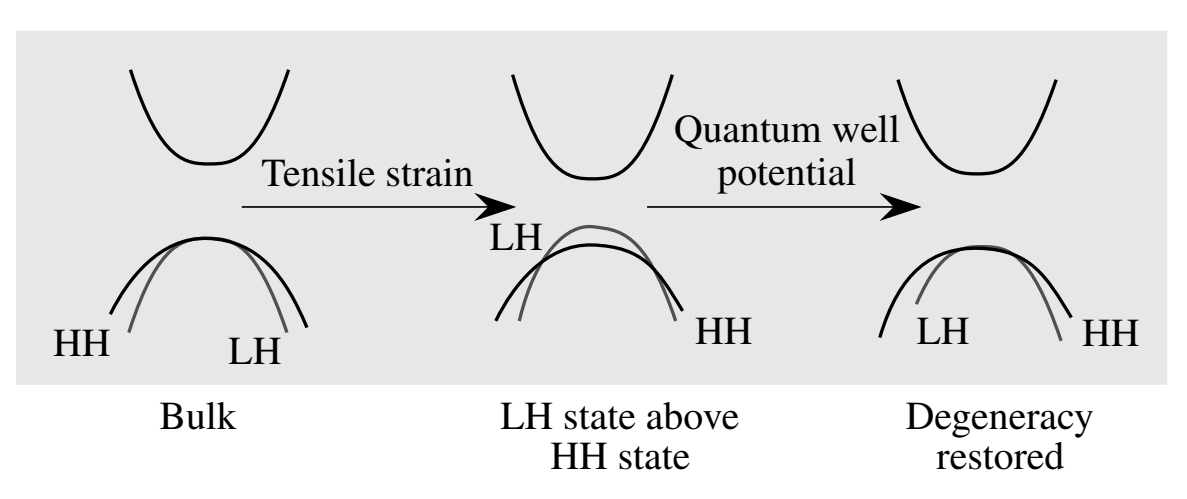
\includegraphics[width=\textwidth]{img/Tensile_Strain.png}
		\\[0.5em]
		\refstepcounter{figure}
		\textbf{Figure~\thefigure.} Effect of biaxial tensile strain and quantum confinement on conduction and valence band states. With appropriate tensile strain, heavy-hole and light-hole states can become degenerate at $\mathbf{k} = 0$ within a quantum well structure.
		\label{fig:tensile_strain}
	\end{minipage}
\end{center}

\subsection{Strained Quantum Wells}
Due to limitations imposed by critical thickness, most strained layers grown by epitaxy are implemented in the form of quantum wells. In these structures, both the effective bandgap and the carrier effective masses are strongly influenced by the presence of strain.\\
As previously discussed, strain—particularly biaxial strain—has a pronounced effect on the valence band edge states. One of the most significant consequences is the reduction of the band-edge density-of-states effective mass. In some cases, the incorporation of strain can lead to a reduction in this mass by nearly a factor of three.
It is evident from the discussion that strain can be a powerful tool for tailoring the electronic bandstructure of semiconductors. The magnitude of strain considered here is readily achievable through strained-layer epitaxy. Importantly, the induced splitting between heavy-hole and light-hole states in the valence band can reach values on the order of 100~meV. Such splitting is accompanied by significant modifications in the band curvature, which directly influence the effective masses and density of states.\\
It is worth noting that achieving similar levels of uniaxial strain through external mechanical means is extremely challenging. The ability to incorporate such strain epitaxially provides a unique and practical avenue for bandstructure engineering.\\
An important question is whether the strain-induced modifications translate into observable changes in physical properties. This topic will be explored in greater depth in later chapters dealing with transport and optical behavior. As will be shown, the effects are indeed substantial and play a key role in the performance of strained semiconductor devices.


\section{Polar Heterostructures}
We have previously discussed that in certain materials, a net polarization can arise due to various mechanisms such as spontaneous polarization, the piezoelectric effect, or ferroelectricity. In face-centered cubic (fcc) semiconductors, spontaneous polarization does not occur; however, strain-induced effects can still lead to a net polarization.\\
One important consequence of polarization differences in semiconductor heterostructures is the emergence of significant built-in electric fields at interfaces. For example, in a polar heterostructure, the interface electric field can be expressed as:
\begin{equation}
	F = \frac{P}{\varepsilon}
\end{equation}
where \( P \) is the net polarization and \( \varepsilon \) is the dielectric constant of the material. This fixed interfacial charge can be harnessed to induce built-in electric fields, generate band bending, and create mobile charge carriers. With proper structural design, this interfacial charge can effectively serve the role of a delta-doping sheet.\\
In zinc blende semiconductors, the piezoelectric effect is the dominant mechanism for polarization. The polarization induced by strain is given in general by:
\begin{equation}
	P_i = \sum_{k,l} e_{ikl} \, \varepsilon_{kl}
\end{equation}
According to Nye (1957), in zinc blende structures only one independent piezoelectric coefficient exists. In the reduced index notation—where \( xx \Rightarrow 1 \), \( yy \Rightarrow 2 \), \( zz \Rightarrow 3 \), \( yz \Rightarrow 4 \), \( zx \Rightarrow 5 \), and \( xy \Rightarrow 6 \)—the only non-zero components of the piezoelectric tensor are:
\begin{equation}
	e_{14} = e_{25} = e_{36}
\end{equation}
This implies that only shear strain contributes to a finite piezoelectric polarization. As previously discussed, in (100) growth the strain tensor is diagonal, and hence, no piezoelectric polarization arises under such epitaxial conditions. However, when growth is performed along directions such as (111), off-diagonal components of the strain tensor become significant. This results in a strong dipole moment across the quantum well, inducing an internal electric field. The corresponding field is given by:
\begin{equation}
	F = \frac{\sqrt{3} e_{14} \, \varepsilon_{xy}}{\varepsilon_s} \quad V/m
\end{equation}
Here, \( e_{14} \) is the piezoelectric coefficient (typically on the order of \( 0.1 \, \text{C/m}^2 \)), \( \varepsilon_{xy} \) is the off-diagonal strain component, and \( \varepsilon_s \) is the dielectric constant. A strain magnitude of approximately 1\% can generate electric fields as high as \( 10^5 \, \text{V/cm} \), highlighting the importance of piezoelectric effects in strained quantum wells.\\
In wurtzite structures (e.g., InN, GaN, AlN), epitaxial growth is typically conducted along the \( c \)-axis, i.e., in the (0001) or \( (\bar{0}001) \) direction. For a sufficiently thick substrate, the in-plane strain components are given by:
\begin{equation}
	\varepsilon_{xx} = \varepsilon_{yy} = \frac{a_3}{a_0} - 1
\end{equation}
where \( a_s \) is the lattice constant of the substrate and \( a_0 \) is that of the unstrained layer. The strain along the growth direction is determined by:
\begin{equation}
	\varepsilon_{zz} = -2 \frac{c_{13}}{c_{33}} \left( \frac{a_s}{a_0} - 1 \right)
\end{equation}
These strains generate a piezoelectric polarization in the strained layer. For wurtzite crystals, the total polarization due to strain is given by:
\begin{equation}
	P_{pz} = e_{33} \varepsilon_{zz} + e_{31} (\varepsilon_{xx} + \varepsilon_{yy})
\end{equation}
where \( e_{33} \) and \( e_{31} \) are piezoelectric constants. The resulting polarization field is directed along the (0001) axis, corresponding to the Ga-face direction in the crystal, following the convention that places Ga atoms on the upper site of each bilayer.\\
The electric field induced by this polarization can be expressed simply as:
\begin{equation}
	F = \frac{P}{\varepsilon_s}
\end{equation}
Typical material constants for InGaN systems include \( c_{13} \approx 109 \, \text{GPa} \) and \( c_{33} \approx 355 \, \text{GPa} \), yielding a ratio \( 2c_{13}/c_{33} \approx 0.6 \). The piezoelectric and spontaneous polarizations play a major role in determining the band alignment and carrier behavior in group-III nitride heterostructures.

\begin{center}
	\begin{minipage}{0.6\textwidth}
		\centering
		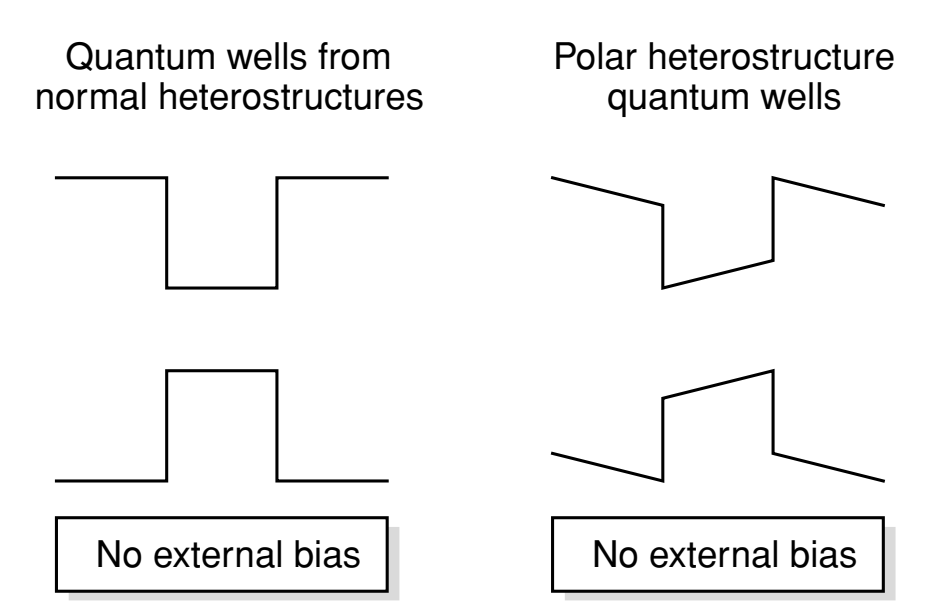
\includegraphics[width=\textwidth]{img/PolarQuantumWell.png}
		\\[0.5em]
		\refstepcounter{figure}
		\textbf{Figure~\thefigure.} A comparison of (undoped) nonpolar and polar quantum well band profiles in the absence of any external electric field.
		\label{fig:polar_quantum_well}
	\end{minipage}
\end{center}